\chapter{DATA C100: Causal Inference and Confouding}

\section{Interpretation of Models}
As previously mentioned, models exist not only for prediction, but also inference. \\
The structure of a model would influence how easy interpretations and inferences can be produced. In this case, since linear regression is a rather conceptually simple model, we will explain the concept of inference using it.

For a linear regression method, we estimate the true relationship between a response and its predictors using a mathematically optimal set of parameters $\hat{\theta}$ specific to the model. \\
That model is:
\[
    f_{\hat{\theta}}(x) = \hat{\theta}_0 + \hat{\theta}_1 x_1 + \cdots + \hat{\theta}_p x_p
\]
Here, the parameters, which essentially have defined the model, is important for inference. \\
For example, if a predictor variable $x_i$ has some estimated parameter of it $\hat{\theta}_i$ that has a zero value, it means the value of $x_i$ does not contribtue to the response variable; therefore, does not affect the response value. \\
We may then test the insignificance of $x_i$ by performing hypothesis testing on the paramter $\theta_i$ as follows:
\begin{bindenum}
    \item \textbf{Null Hypothesis}: The true parameter $\theta_i$ is $0$.
    \item \textbf{Alternate Hypothesis}: The true parameter $\theta_i$ is not $0$.
\end{bindenum}
We will then perform some bootstrapping to produce several models, and see how the confidence interval of estimated parameters $\theta_i$ across each model present. \\
If the confidence interval for our p-value cutoff does indeed involve $0$, we would accept the null hypothesis; otherwise, we find enough reason to reject the null hypothesis.

Is there some mathematical problem that prevents interpretation of invidual predictor variables' significance? Yes. 
If some predicted variables are related to each other, then our interpretation, which attempts to detect the significance of an individual variable with the response, would fail its purpose. \\
We can no longer test one variable by holding others constant, but this is essential to causal inference: inferring whether a specific predictor variable was the cause of some alteration in a response variable. \\
This problem is called \textbf{collinearity}:
\begin{ln-define}{Collinearity}{}
    When a feature can be predicted accurately as a linear function of others, collinearity exists in the dataset. 
    This causes small changes in the data sample to lead to big changes in the estimated slopes of predictor variables. \\
    Collinearity is implied by the noninvertibility of design matrix as well.
\end{ln-define}

\section{Causal Inference}
Here is a short section for outlining the philosophical difference between ``correlation'' (association) and ``causation''.

Questions about correlation look for some mathematical relationship between one variable and another, but causal questions discuss the effects of some intervention. Regression coefficients cannot stand for effects. \\
In other words, correlation questions ask: ``Does the increase of some value coexist with the alteration of some other value, and how significantly?'' \\
But causation would ask: ``Does the increase of some value cause the significant observed alteration of some other values'', and involve counterfactual questions asking if the converse holds true or not to validify the causal effect.

At times, confounding variables appear. \\
A \textbf{confounder} is a variable that affects both the treatment and the response, which distorts the correlation between them. While the common assumption of data science studies would assume that all confounders are observed, confounders can still trigger substantial collinearity in the offered dataset.

Let us now move on to the practical aspects of causal inference. \\
In prediction, we have used the following terminologies:
\begin{bindenum}
    \item \textbf{Response} (Y): what is to be predicted.
    \item \textbf{Predictors} (X): what is to be inputted.
\end{bindenum}
But, in causal inference, we will modify these terminologies slightly along the context of inference problems:
\begin{bindenum}
    \item \textbf{Response} (Y): the outcome of interest.
    \item \textbf{Treatment} (T): the variable we might intervene on.
    \item \textbf{Covariate} (X): potential confounders.
\end{bindenum}
For the scope of this course, we will focus on $T$ as indicator variables. \\
Each datapoint of our model will then be involved as tuples of following format:
\[
    (x_i, T_i, Y_i (0), Y_i (1))
\]
where the variables respectively stand for covariates, treatment, treated outcome ($y_i$ if $T_i = 1$), and control outcome ($y_i$ if $T_i = 0$). \\
This model is known as the \textbf{Neyman-Rubin Causal Model}. However, since we only ever observe one of the potential outcome (treated or control). There are limitations upon which we estimate the true effects of a treatment. \\
For example, on the metric \textbf{Average Treatment Effect}:
\[ATE = \E[Y(1)] - \E[Y(0)]\]
we cannot just take a sample mean as an estimator, because we only ever observe one potential outcome per datapoint.

Now, how do we assign treatments to different groups to avoid statistical bias? \\
While randomized experiments are theoretically suitable approaches, they are often unethical or impractical in realistic contexts. Therefore, scientists have long preferred its alternative: \textbf{observational studies}. \\
In observational studies, we merely observe the effects of treatments without much priori or beforehand knowledge on possible inherent deviations between ``treatment group'' and ``control group''. This develops into unmeasured confounders, which also do not appear ideal for accurate inferences. \\
But, in other words, we now just have to find a way to mitigate confounders.

\section{Covariate Adjustment}
The aforementioned great assumption for confounders has been \textbf{ignorability assumption}; once again, it states that all important confounders are in the data set. \\
However, such approach is very fragile: it breaks if important covariates are missing, or if the true dependence on $x$ is nonlinear. \\
Albeit we may also come up with some model that ought to include them, additional ssumptions would be needed for the model to finally work.

There still exist other methods for alleviating confounders, where many of these methods would model treatment as a function of covariates, if not modeling the outcome as a function of both covariate and treatment. \\
One notable example, meanwhile, would be regression discontinuity. Such a method has a running variable $x$, and let $T = 1$ if and only iff $x > \text{threshold}$. This would allow us to have two separate regression models piecewise-concatenated together. \\
This method would avoid the confounding issues as treatment becomes a determinstic function of covariates, estimand becomes ATE for units near the threshold, and is widely used across real-life problems such as clinical threshold for treatment and PSAT/NMSQT cutoffs.
\begin{ln-fig}{Regression Discontinuity, DATA C100}{}
    \begin{center}
        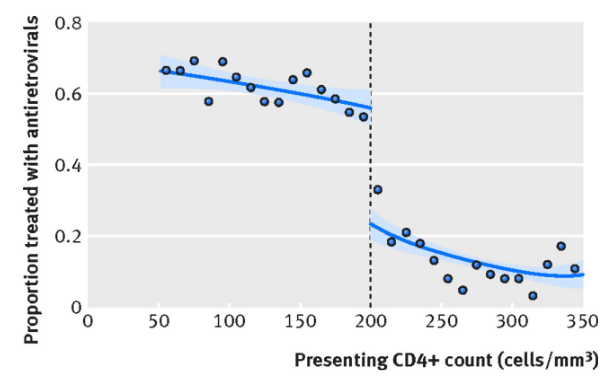
\includegraphics[scale=0.8]{figs/ln10/reg-discont.png}
    \end{center}
\end{ln-fig}
